\documentclass[10pt]{article}
\usepackage[hmargin=0.8in,vmargin=0.65in]{geometry}
\usepackage{amsmath,amssymb}
\usepackage{longtable,booktabs,array}
\usepackage{graphicx}
\graphicspath{{../figures/}{plans/active/figures/}{figures/}}
\usepackage{algorithm}
\usepackage{algpseudocode}
\makeatletter
\renewenvironment{algorithm}[1][]{%
  \par\addvspace{8pt}%
  \renewcommand{\caption}[1]{\refstepcounter{algorithm}\noindent\textbf{Algorithm \thealgorithm}\enspace ##1\par\nobreak\vskip2pt}%
  \hrule\nobreak\vskip2pt%
}{%
  \par\nobreak\vskip2pt\hrule\addvspace{8pt}%
}
\makeatother
\algrenewcommand\algorithmicrequire{\textbf{Input:}}
\algrenewcommand\algorithmicensure{\textbf{Output:}}
\usepackage[hidelinks]{hyperref}
% Compact spacing without shrinking equations or plot labels.
\setlength{\textfloatsep}{10pt plus 2pt minus 2pt}
\setlength{\floatsep}{8pt plus 2pt minus 2pt}
\setlength{\intextsep}{8pt plus 2pt minus 2pt}
\setlength{\abovecaptionskip}{4pt}
\setlength{\belowcaptionskip}{0pt}
\setlength{\LTpre}{4pt}
\setlength{\LTpost}{4pt}
\renewcommand{\topfraction}{0.9}
\renewcommand{\bottomfraction}{0.85}
\renewcommand{\textfraction}{0.08}
\renewcommand{\floatpagefraction}{0.8}
\raggedbottom
\setcounter{topnumber}{4}
\setcounter{bottomnumber}{3}
\setcounter{totalnumber}{6}
\makeatletter
\renewcommand\section{\@startsection{section}{1}{\z@}{-1.6ex plus -.4ex}{.7ex}{\normalfont\large\bfseries}}
\renewcommand\subsection{\@startsection{subsection}{2}{\z@}{-1.1ex plus -.3ex}{.5ex}{\normalfont\normalsize\bfseries}}
\makeatother
\AtBeginDocument{%
  \setlength{\abovedisplayskip}{6pt plus 2pt minus 2pt}%
  \setlength{\belowdisplayskip}{6pt plus 2pt minus 2pt}%
  \setlength{\abovedisplayshortskip}{3pt}%
  \setlength{\belowdisplayshortskip}{4pt}%
}
\title{Project Update: Multi-Agent Housing and Insurance Market}
\author{Neil Dhawan, Jon Legasa, Alejandro Ordonez}
\date{October 28, 2026}

\makeatletter
\renewcommand{\maketitle}{%
\begin{center}
{\Large\bfseries \@title\par}
\vspace{4pt}
\@author\par
\vspace{4pt}
\@date\par
\end{center}
}
\makeatother

\begin{document}
\maketitle

\begin{abstract}
We have constructed a housing and insurance environment for Q-learning agents using Lorenz allocations of income and ownership, spatially correlated home prices, and income-dependent residence assignment. Poisson disasters destroy homes within fixed zones, linking property losses and displacement to insurance claims. The proposed spatial extension assigns hidden regional risk that agents learn from public disaster histories. Three experimental worlds---``Peace'', ``Standard'', and ``Chaos''---compare equal and unequal initial resources under constant or increasing disaster rates.
\end{abstract}

\section{Market model}
Agents act as renters, owner-occupiers, or landlords; insurers offer coverage. Their decisions connect ownership, rent, insurance purchases, and claims.

Lorenz curves control income and ownership inequality. A shared ranking associates higher income with larger intended portfolios. Spatial price variation and noisy residence assignment create neighborhoods with different wealth and exposure.

Disasters produce losses across neighboring homes, exposing owners, residents, and insurers to the same event.

\begin{figure}[H]
\centering
\setlength{\unitlength}{1pt}
\begin{picture}(430,135)
\put(5,97){\framebox(115,28){\shortstack{Agent 1\\Owner-occupier}}}
\put(157,97){\framebox(115,28){\shortstack{Agent 2\\Landlord}}}
\put(310,97){\framebox(115,28){\shortstack{Agent 3\\Renter}}}
\put(5,5){\framebox(115,28){\shortstack{Home A\\Residence of agent 1}}}
\put(255,5){\framebox(170,28){\shortstack{Home B\\Residence of agent 3}}}
\put(62,97){\vector(0,-1){64}}
\put(68,57){\makebox(90,16)[l]{\small Owns and occupies}}
\put(214,97){\line(0,-1){44}}
\put(214,53){\line(1,0){77}}
\put(291,53){\vector(0,-1){20}}
\put(231,57){\makebox(45,14){\small Owns}}
\put(367,97){\vector(0,-1){64}}
\put(371,57){\makebox(55,16)[l]{\small Occupies}}
\put(310,111){\vector(-1,0){38}}
\put(270,118){\makebox(39,14){\small Rent}}
\end{picture}
\caption{Housing relationships: agent 1 owns their residence; agent 3 rents from agent 2. Roles can overlap or change.}
\label{fig:housing-market}
\end{figure}

\section{Model assumptions}
\label{sec:assumptions}

\begin{itemize}
\item \textbf{Agents and objectives.} Individual and insurer agents use Q-learning to maximize expected discounted cumulative rewards. Renter, owner-occupier, and landlord are housing relationships, not fixed agent types.
\item \textbf{Housing and allocation.} Each grid cell is one home. The population and housing supply are fixed and equal, with one resident per home initially. Ownership is separate from residence and may be concentrated. Initial allocation does not enforce affordability. Initial prices are positive; rent and starting capital are configured separately.
\item \textbf{Income and inequality.} External income is assigned once, accrues each period, and is paid every 10 completed simulation runs; landlords receive accrued rent every 20 completed runs. Section~\ref{sec:payment-schedule} defines the payment clock. Jobs are not simulated. Income and ownership curves share a agent ranking. Recurring income adds money to the economy. ``Peace'' imposes equal initial resources, with no ongoing wealth cap or redistribution.
\item \textbf{Spatial fields.} Seeded noise generates initial prices and a separate disaster-risk field. The risk field is independent of initial prices and remains fixed during an episode. Spatial boundaries do not wrap. A global seed supplies separate random streams for reproducible runs.
\item \textbf{Disaster occurrence.} Each period, draw the number of disasters from a Poisson distribution. Choose each disaster location independently using the hidden risk map. Every event affects a rectangle of the same size, entirely within the grid. The event rate may change over time; the risk map and rectangle size stay fixed.
\item \textbf{Public information.} After each disaster, every agent and insurer observes its time, affected cells, and resulting housing damage across the grid. The underlying risk field and location probabilities are not provided to agents. They can learn about regional risk from the shared event history, including events outside their own holdings.
\item \textbf{Damage and recovery.} An affected intact home loses all modeled value and becomes uninhabitable. Its resident is displaced and its owner retains title. Surviving land value, rebuilding, and replacement housing are omitted. Repeated damage to an already destroyed home generates no new building loss.
\item \textbf{Insurance and timing.} Coverage is chosen before exposure, with up-front premiums and fixed contract terms. Income and rent accrue during each run and settle on their scheduled run boundaries; when both are due, income is paid before rent. Disasters and claims continue within each run. Claims use pre-loss building values or specified contents amounts, subject to deductibles, coverage limits, and available insurer capital. Capital shortfalls are recorded; claims are settled after each event.
\end{itemize}

\section{Environment and notation}
The $m\times n$ grid contains $H=mn$ homes, $N=H$ agents, and $F$ insurers. Matrices index homes by location; vectors index agents.

\subsection{Definitions and glossary}
Let $i$ index agents, $t$ simulation periods, and $(a,b)$ and $(u,v)$ home locations. Their domains are
\begin{equation}
\begin{aligned}
 m,n,N,F &\in\mathbb{Z}_{>0}, & H&=mn,\\
 i &\in\{1,\ldots,N\}, & t&\in\mathbb{Z}_{\geq0},\\
 (a,b),(u,v) &\in\{1,\ldots,m\}\times\{1,\ldots,n\}.
\end{aligned}
\end{equation}
Quantities are current unless stated otherwise.

\begingroup
\renewcommand{\arraystretch}{1.0}
\setlength{\LTpre}{2pt}
\setlength{\LTpost}{2pt}
\begin{longtable}{@{}p{0.17\textwidth}>{\raggedright\arraybackslash}p{\dimexpr0.83\textwidth-2\tabcolsep\relax}@{}}
\toprule
\textbf{Symbol} & \textbf{Meaning} \\
\midrule
\endfirsthead
\toprule
\textbf{Symbol} & \textbf{Meaning (continued)} \\
\midrule
\endhead
\bottomrule
\endfoot
$P$ & $\mathbb{R}_{\geq0}^{m\times n}$. Home values. \\
$O$ & $\{1,\ldots,N\}^{m\times n}$. Owners, represented by agent indices. \\
$R$ & $\{0,\ldots,N\}^{m\times n}$. Residents; zero denotes vacancy. \\
$D$ & $\{0,1\}^{m\times n}$. Destruction indicators; one denotes an uninhabitable home. \\
$\mathbf{y}$ & $\mathbb{R}_{\geq0}^{N}$. Fixed annual external incomes. \\
$\mathbf{c}$ & $\mathbb{R}_{\geq0}^{N}$. Cash balances. \\
\end{longtable}

Initially, $P\in\mathbb{R}_{>0}^{m\times n}$, $D=0$, and each agent appears once in $R$. Ownership indices may repeat. A tenancy occurs where $R_{ab}>0$ and $R_{ab}\ne O_{ab}$. After displacement, a agent may have no residence.

The ownership indicator $\mathbf{1}_{\{O_{ab}=i\}}$ identifies homes belonging to agent $i$. Their home count and property wealth are
\begin{equation}
\begin{aligned}
 \text{home count of agent }i &= \sum_{a=1}^{m}\sum_{b=1}^{n}\mathbf{1}_{\{O_{ab}=i\}},\\
 \text{property wealth of agent }i &= \sum_{a=1}^{m}\sum_{b=1}^{n}P_{ab}\mathbf{1}_{\{O_{ab}=i\}}.
\end{aligned}
\end{equation}

\begingroup
\makeatletter\def\@captype{figure}\makeatother
\[
\underbrace{\begin{bmatrix}200&300\\400&500\end{bmatrix}}_{P\text{ (thousands)}}
\qquad
\underbrace{\begin{bmatrix}3&4\\3&4\end{bmatrix}}_{O\text{ (owners)}}
\qquad
\underbrace{\begin{bmatrix}1&2\\3&4\end{bmatrix}}_{R\text{ (residents)}}
\]
\caption{Illustrative allocation: agents 1 and 2 rent from 3 and 4. Each owner holds two homes, worth 600 and 800 thousand respectively.}
\label{fig:matrices}
\endgroup

Contracts link agents, insurers, homes, and coverage terms.

\subsection{Learning terminology and notation}
The proposed tabular Q-learning specification in Section~\ref{sec:rl-agents} uses \emph{household} for an individual agent and \emph{firm} for an insurer. These are the two learner types; housing roles describe a household's relationship to homes. Reinforcement learning (RL) updates action values from rewards observed through interaction with the environment. A tabular Q-learner stores these values in a table indexed by state and action.

\begin{longtable}{@{}p{0.17\textwidth}>{\raggedright\arraybackslash}p{\dimexpr0.83\textwidth-2\tabcolsep\relax}@{}}
\toprule
\textbf{Symbol or term} & \textbf{Meaning} \\
\midrule
\endfirsthead
\toprule
\textbf{Symbol or term} & \textbf{Meaning (continued)} \\
\midrule
\endhead
\bottomrule
\endfoot
$k$ & $\{h,f\}$. Learner type: household ($h$) or insurer ($f$); these superscripts label types. \\
$j$ & $\{1,\ldots,F\}$. Insurer index in the learning specification. \\
$s,s'$ & Type-specific states. Current and next state; $s_i^h$ and $s_j^f$ denote household and insurer states. \\
$\mathcal{A}^k$ & Type-specific action set. Actions for learner type $k$; $a$ is the chosen action and $a'$ indexes candidate next actions. Here $a$ denotes an action, rather than a grid coordinate. \\
$Q^k(s,a)$ & $\mathbb{R}$. Estimated discounted return for a state--action pair, stored in the shared table for type $k$. \\
$\alpha$ & $(0,1]$. Learning rate controlling the size of a Q-value update. \\
$\gamma$ & $[0,1]$. Discount factor weighting future rewards. \\
$\varepsilon$ & $[0,1]$. Exploration probability in $\varepsilon$-greedy action selection; otherwise an action with maximal Q-value is selected. \\
$r,r_i^h,r_j^f$ & $\mathbb{R}$. Immediate reward, with household and insurer forms defined in the learning specification. \\
$\Delta$ & Change operator. Change in a quantity over a period, as used in the household reward. \\
$\kappa,\kappa_f$ & $\mathbb{R}_{\geq0}$. Household displacement and insurer insolvency penalties. \\
$r_f$ & $\mathbb{R}_{\geq0}$. Risk-free rate applied to insurer capital per period; distinct from the insurer reward $r_j^f$. \\
Pure premium & Expected loss cost. Fitted loss cost used as the reference for the insurer's premium ladder. \\
Tweedie GLM & Statistical model. Tweedie generalized linear model used in the proposed offline pure-premium fit. \\
\end{longtable}

\subsection{Distribution functions and parameters}
\begin{longtable}{@{}p{0.17\textwidth}>{\raggedright\arraybackslash}p{\dimexpr0.83\textwidth-2\tabcolsep\relax}@{}}
\toprule
\textbf{Symbol} & \textbf{Definition} \\
\midrule
\endfirsthead
\toprule
\textbf{Symbol} & \textbf{Definition (continued)} \\
\midrule
\endhead
\bottomrule
\endfoot
$L_y,L_h$ & $[0,1]\to[0,1]$. Lorenz functions for income and home counts along the same agent ordering. \\
$\mu$ & $\mathbb{R}_{>0}$. Mean annual external income. \\
$\Delta t$ & $\mathbb{R}_{>0}$. Period length in years. \\
$q$ & $\mathbb{Z}_{\geq0}$. Completed simulation runs in a payment sequence; each run contains $T$ periods. \\
$I_q,J_q$ & $\{0,1\}$. Income and rent payment indicators at run boundary $q$, defined in Section~\ref{sec:payment-schedule}. \\
$p_0$ & $\mathbb{R}_{>0}$. Reference home price. \\
$\sigma,\ell$ & $\mathbb{R}_{\geq0}$. Log-price variation and spatial smoothing scale. \\
$\tau$ & $\mathbb{R}_{\geq0}$. Noise strength for residence placement. \\
$\lambda_t$ & $\mathbb{R}_{\geq0}$. Expected disasters in period $t$. \\
$S$ & $\mathbb{Z}_{\geq0}$. Global seed for labeled component random streams. \\
\end{longtable}

Agents are indexed by nondecreasing income, with seeded tie-breaking.

\endgroup

\section{Assigning initial home values}
\label{sec:home-values}
Let $E\in\mathbb{R}^{m\times n}$ be the seeded noise matrix used to generate home prices:
\begin{equation}
 E_{ab}\overset{\mathrm{iid}}{\sim}\mathcal{N}(0,1).
\end{equation}
\begin{figure}[H]
\centering
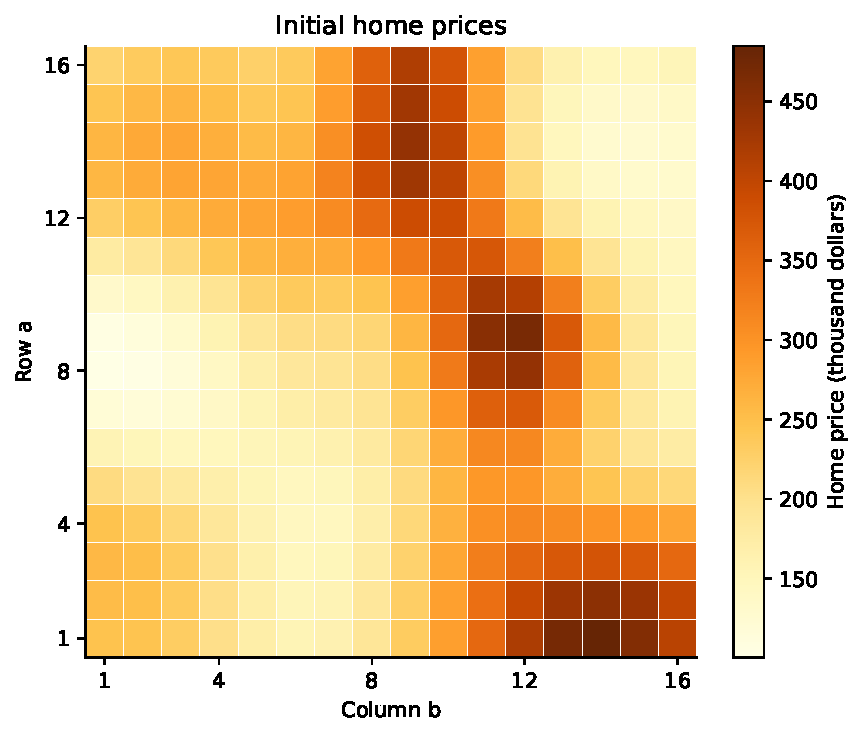
\includegraphics[width=0.48\textwidth]{initial-prices.pdf}
\caption{Each cell is one home; color shows its initial price generated from seeded spatial noise. Example: $m=n=16$, $S=42$, $p_0=250{,}000$, $\sigma=0.4$, $\ell=2$.}
\label{fig:price-distribution}
\end{figure}

\textit{We reuse this smoothing operator for disaster risk in Section~\ref{sec:hidden-risk}.} For scale $\ell>0$, let $w_{ab,uv}$ weight cell $(u,v)$ at location $(a,b)$. Define $\mathcal{S}_{\ell}$ by
\begin{equation}
\begin{aligned}
 w_{ab,uv}
 &=\exp\left(-\dfrac{(a-u)^2+(b-v)^2}{2\ell^2}\right),\\[8pt]
 [\mathcal{S}_{\ell}(E)]_{ab}
 &=\dfrac{\displaystyle\sum_{u=1}^{m}\sum_{v=1}^{n}w_{ab,uv}E_{uv}}
 {\displaystyle\sqrt{\sum_{u=1}^{m}\sum_{v=1}^{n}w_{ab,uv}^{2}}}.
\end{aligned}
\end{equation}
The scale $\ell$ controls neighborhood size; normalization gives unit variance at each cell. Set $\mathcal{S}_0(E)=E$ for no smoothing.

Using reference price $p_0$ and log-price spread $\sigma$, the initial price matrix is
\begin{equation}
 P=p_0\exp\left(\sigma\mathcal{S}_{\ell}(E)\right).
\end{equation}
\begin{algorithm}[H]
\caption{Generate initial home values}
\label{alg:prices}
\begin{algorithmic}[1]
\Require Grid dimensions, $p_0,\sigma,\ell$, and seeded price stream
\State Draw $E_{ab}\overset{\mathrm{iid}}{\sim}\mathcal{N}(0,1)$
\State $P\gets p_0\exp\bigl(\sigma\mathcal{S}_{\ell}(E)\bigr)$; $D\gets0$
\State \Return $P,D$
\end{algorithmic}
\end{algorithm}

The entrywise exponential gives positive prices with median $p_0$ at each cell. Prices are independent of population allocation and rounded to cents.



\section{Assigning income and ownership shares}
The Lorenz curves $L_y$ and $L_h$ allocate $N\mu$ annual income and $H$ homes along a shared income ranking. Separate curves control income and ownership concentration.

\begin{figure}[H]
\centering
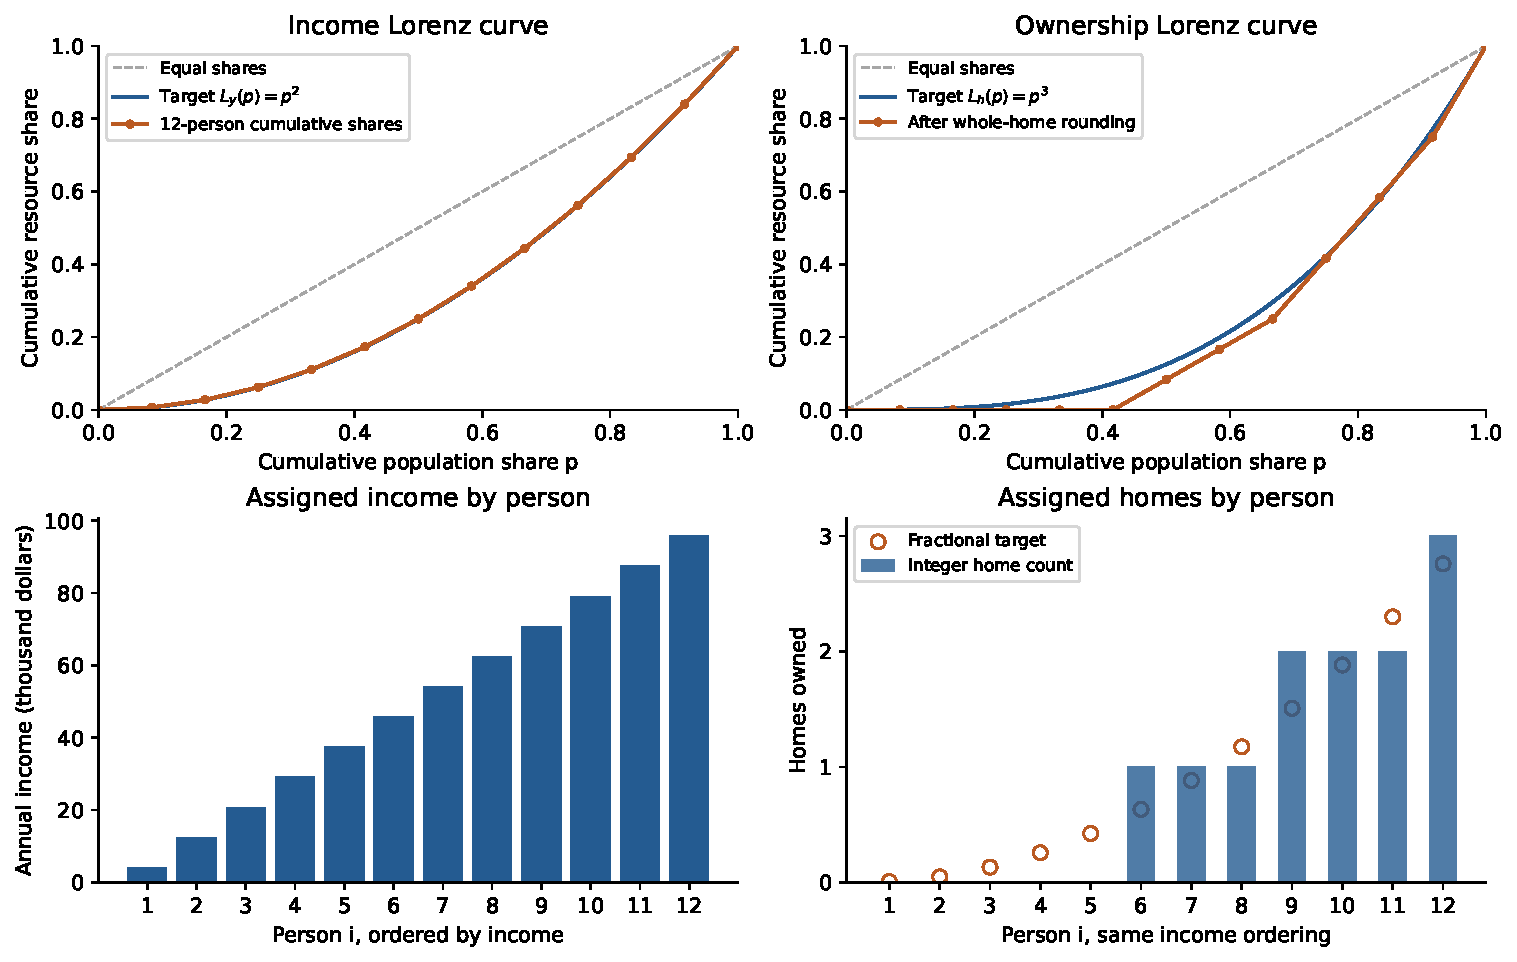
\includegraphics[width=0.88\textwidth]{lorenz-allocations.pdf}
\caption{Illustrative allocation: $N=H=12$, $\mu=50{,}000$, $L_y(p)=p^2$, $L_h(p)=p^3$. Markers show finite-population shares; lower panels show incomes and integer home counts against fractional targets.}
\label{fig:lorenz-distributions}
\end{figure}

For $L\in\{L_y,L_h\}$, let $\mathbf{d}(L)\in[0,1]^N$ contain individual shares:
\begin{equation}
 [\mathbf{d}(L)]_i
 =L\left(\dfrac{i}{N}\right)
 -L\left(\dfrac{i-1}{N}\right),
 \qquad i\in\{1,\ldots,N\}.
\end{equation}
Let $y_i$ be annual income and $a_i$ the fractional home target for agent $i$:
\begin{equation}
\begin{aligned}
 y_i&=N\mu\left[
 L_y\left(\dfrac{i}{N}\right)-L_y\left(\dfrac{i-1}{N}\right)
 \right],\\[3pt]
 a_i&=H\left[
 L_h\left(\dfrac{i}{N}\right)-L_h\left(\dfrac{i-1}{N}\right)
 \right].
\end{aligned}
\end{equation}
Let $\mathbf{a}\in\mathbb{R}_{\geq0}^{N}$ collect fractional targets and $\mathbf{h}\in\mathbb{Z}_{\geq0}^{N}$ whole-home allocations. Round and correct the total:
\begin{enumerate}
\item Round each $a_i$ to the nearest integer, rounding halves upward.
\item If $\sum_i h_i<H$, add one to the count with largest $a_i-h_i$.
\item If $\sum_i h_i>H$, subtract one from a positive count with largest $h_i-a_i$.
\end{enumerate}
\begin{algorithm}[H]
\caption{Assign incomes and home counts}
\label{alg:incomes}
\begin{algorithmic}[1]
\Require $N,H,\mu,L_y,L_h$ and seeded tie-breaking
\State $\mathbf{y}\gets N\mu\mathbf{d}(L_y)$; $\mathbf{a}\gets H\mathbf{d}(L_h)$
\State Round each $a_i$ to the nearest integer $h_i$, with halves rounded upward
\State Correct largest rounding residuals until $\sum_i h_i=H$, as specified above
\State \Return $\mathbf{y},\mathbf{h}$
\end{algorithmic}
\end{algorithm}

Repeat until $\sum_i h_i=H$, recomputing residuals and breaking ties by seed. Ownership shares target home counts, not property values.



\subsection{Payment schedule across simulation runs}
\label{sec:payment-schedule}
Let $q$ count completed simulation runs (episodes), each lasting $T\Delta t$ years. Income is paid every 10 runs and rent every 20:
\begin{equation}
\begin{aligned}
 I_q&=\mathbf{1}_{\{q>0\ \text{and}\ q\bmod 10=0\}},
 & &\text{income payment},\\
 J_q&=\mathbf{1}_{\{q>0\ \text{and}\ q\bmod 20=0\}},
 & &\text{rent payment}.
\end{aligned}
\end{equation}
Income accumulates between paydays:
\begin{equation}
 \mathbf{c}\gets\mathbf{c}+I_q\,(10T\Delta t)\,\mathbf{y}.
\end{equation}
When $J_q=1$, tenants transfer accrued rent to their landlords, after income is credited. Cash and unpaid balances carry between runs; independent sequences start at $q=0$ with no payment due. Rent amounts and insufficient-cash rules remain open.



\section{Connecting agents to homes}
Residences are assigned by income with random variation; ownership is assigned separately.

For agent $i$, let $B_i$ contain agents with lower income and $T_i$ contain agents with the same income:
\[
\begin{aligned}
 B_i &:= \{j\in\{1,\ldots,N\}:y_j<y_i\},
 & &\text{lower-income agents},\\[5pt]
 T_i &:= \{j\in\{1,\ldots,N\}:y_j=y_i\},
 & &\text{equal-income agents}.
\end{aligned}
\]
Let $r_i\in[0,1]$ be the income percentile, $z_i\in\mathbb{R}$ an independent noise draw, and $q_i\in\mathbb{R}$ the placement score. Using $|B_i|$ and $|T_i|$ for the respective group sizes, define
\begin{equation}
\begin{aligned}
 r_i &:= \dfrac{|B_i|+\dfrac{1}{2}|T_i|}{N},
 & &\text{income percentile},\\[8pt]
 z_i &\overset{\mathrm{iid}}{\sim}\mathcal{N}(0,1),
 & &\text{placement noise},\\[5pt]
 q_i &:= r_i+\tau z_i,
 & &\text{placement score}.
\end{aligned}
\end{equation}
Match agents ranked by $\mathbf{q}$ to homes ranked by price. Equal incomes receive equal percentiles; ties are broken by seed. Increasing $\tau$ weakens income-based sorting. An independent baseline uses random assignment.

Each agent with $h_i>0$ first owns their residence. Shuffle the remaining owner-capacity slots across unassigned titles. Larger residual quotas receive proportionally more titles; agents with $h_i=0$ become renters.

\begin{algorithm}[H]
\caption{Assign residences and ownership}
\label{alg:board}
\begin{algorithmic}[1]
\Require $P,\mathbf{y},\mathbf{h},\tau$ and seeded placement and ownership streams
\State Compute income percentiles $\mathbf{r}$ and draw $z_i\overset{\mathrm{iid}}{\sim}\mathcal{N}(0,1)$
\State Match agents ranked by $q_i=r_i+\tau z_i$ to cells ranked by price, filling $R$
\State Give each agent with $h_i>0$ ownership of their residence
\State Shuffle residual owner-capacity slots and assign remaining titles, filling $O$
\State \Return $R,O$
\end{algorithmic}
\end{algorithm}

\section{Insurance coverage and claims}
Insurers offer homeowners, landlord, and renters coverage. The opening round collects offers and coverage choices before exposure. Fixed quotes and cheapest-affordable purchases provide reference policies for learned pricing and purchasing.

For a covered claim, let $x\geq0$ be the loss amount, $\delta\geq0$ the deductible, and $L_{\max}\geq0$ the coverage limit. Let $b_f\geq0$ be insurer $f$'s available capital immediately before payment, with $f\in\{1,\ldots,F\}$. All amounts are in dollars.

Let $C_{\mathrm{due}}$ denote the contractual payment, $C_{\mathrm{paid}}$ the actual payment, and $C_{\mathrm{short}}$ the unpaid contractual amount:
\begin{equation}
\begin{aligned}
 C_{\mathrm{due}}&=\min\!\left\{L_{\max},\max\{0,x-\delta\}\right\},
 & &\text{payment due},\\[6pt]
 C_{\mathrm{paid}}&=\min\{C_{\mathrm{due}},b_f\},
 & &\text{payment made},\\[6pt]
 C_{\mathrm{short}}&=C_{\mathrm{due}}-C_{\mathrm{paid}},
 & &\text{capital shortfall}.
\end{aligned}
\end{equation}
For a claim on home $(a,b)$, let $P_{ab}^{\mathrm{pre}}$ be its value immediately before destruction and $v_{\mathrm{contents}}\geq0$ the contract's contents-loss amount. Under the total-loss rule,
\begin{equation}
 x=\begin{cases}
 P_{ab}^{\mathrm{pre}}, & \text{homeowners or landlord building claim},\\[4pt]
 v_{\mathrm{contents}}, & \text{renters contents claim}.
 \end{cases}
\end{equation}
For insured agent $i$, settlement transfers the payment:
\begin{equation}
\begin{aligned}
 b_f&\gets b_f-C_{\mathrm{paid}},
 & &\text{insurer capital},\\[4pt]
 c_i&\gets c_i+C_{\mathrm{paid}},
 & &\text{insured agent cash}.
\end{aligned}
\end{equation}
Claims are settled in contract-ID order using the remaining capital for each payment.

\begin{figure}[H]
\centering
\setlength{\unitlength}{1pt}
\begin{picture}(430,155)
\put(5,120){\framebox(125,28){\shortstack{Owner-occupier\\Homeowners coverage}}}
\put(152,120){\framebox(125,28){\shortstack{Landlord\\Landlord coverage}}}
\put(299,120){\framebox(125,28){\shortstack{Renter\\Renters coverage}}}
\put(67,120){\line(0,-1){15}}
\put(214,120){\line(0,-1){15}}
\put(361,120){\line(0,-1){15}}
\put(67,105){\line(1,0){294}}
\put(130,105){\vector(0,-1){57}}
\put(35,70){\makebox(85,18){\small Premiums}}
\put(330,48){\vector(0,1){57}}
\put(163,65){\makebox(155,30){\shortstack{\small Offers and covered\\\small claim payments}}}
\put(5,0){\framebox(419,48){}}
\put(10,30){\makebox(409,15){\small Competing insurer RL agents}}
\put(20,6){\framebox(115,20){Firm A}}
\put(157,6){\framebox(115,20){Firm B}}
\put(294,6){\framebox(115,20){Firm C}}
\end{picture}
\caption{Housing roles determine applicable coverage. Agents choose among competing firms; arrows represent market access and contractual payments.}
\label{fig:insurance-market}
\end{figure}

Owners and tenants may insure different losses at the same home with different firms.

\begin{algorithm}[H]
\caption{Open the insurance market}
\label{alg:insurance}
\begin{algorithmic}[1]
\Require Housing allocation, cash, insurer capital, and decision policies
\State Collect all insurer offers, then each agent's coverage choices
\State Validate eligibility and affordability; transfer accepted premiums
\State Activate contracts and return updated balances
\end{algorithmic}
\end{algorithm}

\section{Disaster occurrence and damage}
Each disaster affects a fixed rectangular zone. Intact homes within it lose all modeled value and become uninhabitable; homes outside it are unaffected.

\begin{figure}[H]
\centering
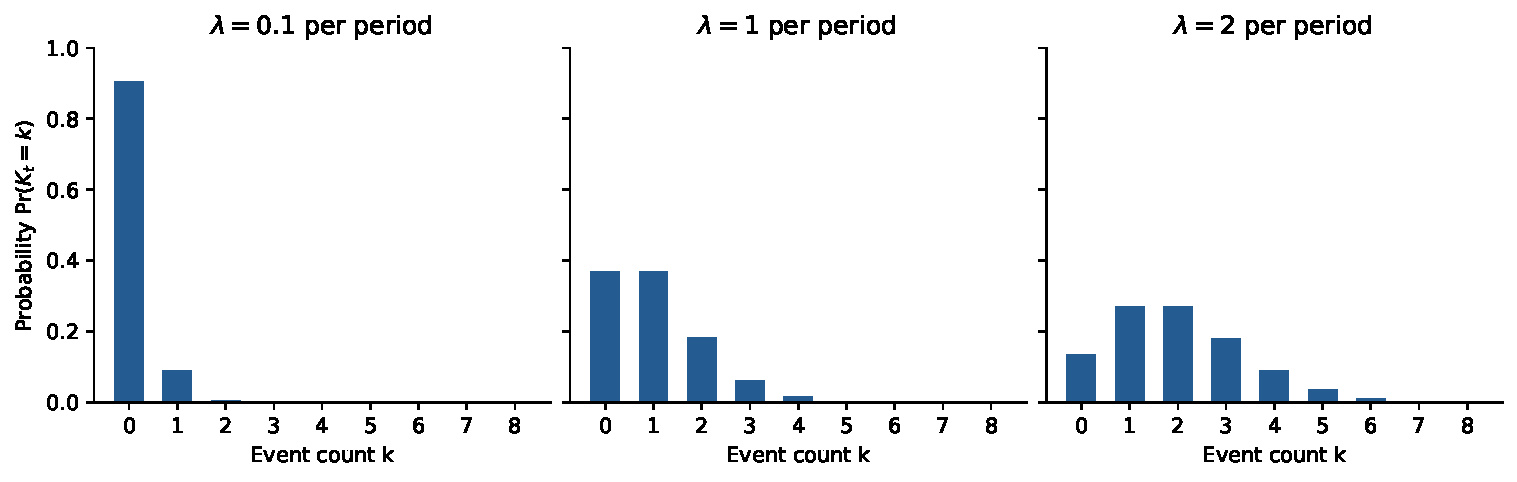
\includegraphics[width=\textwidth]{poisson-counts.pdf}
\caption{Disaster counts per period for illustrative rates, not selected simulation parameters. Displayed probability masses cover $k\in\{0,\ldots,8\}$; the omitted tail is below $0.00024$ in each panel.}
\label{fig:poisson-distribution}
\end{figure}

Let $K_t\in\mathbb{Z}_{\geq0}$ count disasters in period $t$, with mean $\lambda_t$, and let $f(k;\lambda_t)$ be its probability mass function. Counts are independent conditional on the rate schedule:
\begin{equation}
\begin{aligned}
 K_t&\sim\operatorname{Poisson}(\lambda_t),\\[3pt]
 f(k;\lambda_t)
 &=\Pr(K_t=k)
 =\dfrac{\lambda_t^k e^{-\lambda_t}}{k!},
 \qquad k\in\mathbb{Z}_{\geq0}.
\end{aligned}
\end{equation}
At $\lambda_t=0$, $\Pr(K_t=0)=1$.

\subsection{Hidden spatial risk}
\label{sec:hidden-risk}
An anchor is a disaster zone's upper-left cell. Let $\mathcal{A}$ contain anchors whose entire footprint fits within the grid.

\begin{figure}[H]
\centering
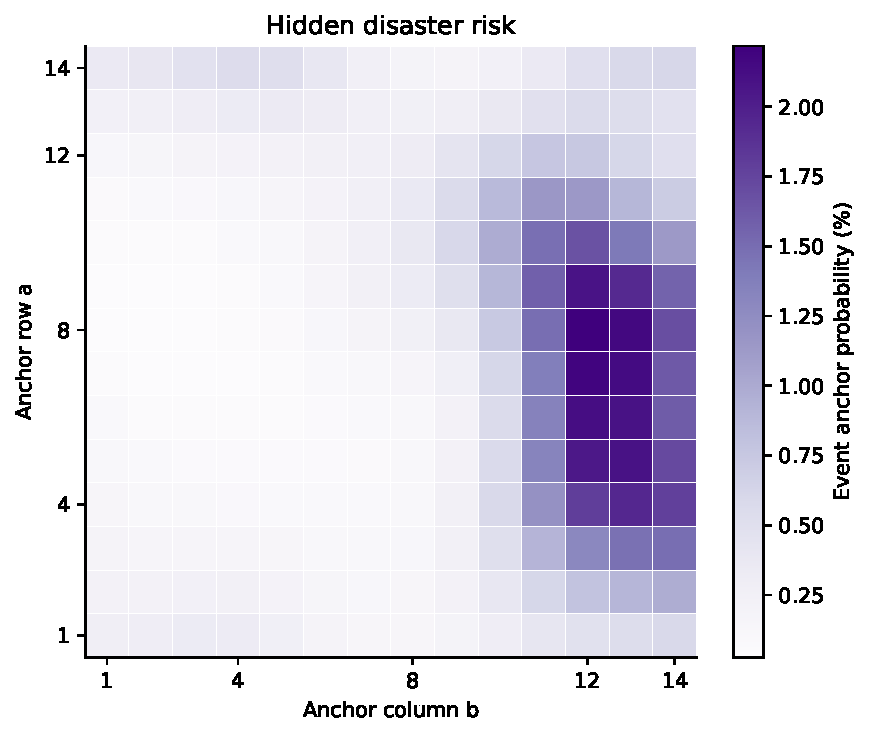
\includegraphics[width=0.48\textwidth]{hidden-spatial-risk.pdf}
\caption{Darker purple denotes higher anchor probability. Example: $16\times16$ homes, a $3\times3$ footprint, $14\times14$ eligible anchors, $S=42$, $\eta=1$, $\ell_{\mathrm{risk}}=2$. This risk map is hidden from agents.}
\label{fig:hidden-spatial-risk}
\end{figure}

Let $U\in\mathbb{R}^{m\times n}$ be seeded Gaussian noise independent of price noise, $\ell_{\mathrm{risk}}\geq0$ the smoothing scale, and $\eta\geq0$ the risk contrast. Reusing $\mathcal{S}$ from Section~\ref{sec:home-values}, define the positive weight field $V$:
\begin{equation}
\begin{aligned}
 U_{ab}&\overset{\mathrm{iid}}{\sim}\mathcal{N}(0,1),
 & &\text{risk noise},\\[5pt]
 V_{ab}&=\exp\!\left(\eta[\mathcal{S}_{\ell_{\mathrm{risk}}}(U)]_{ab}\right),
 & &\text{spatial weight}.
\end{aligned}
\end{equation}
Let $\pi_{ab}$ be the probability of selecting anchor $(a,b)\in\mathcal{A}$, and $\lambda_t(a,b)$ its expected event count in period $t$:
\begin{equation}
\begin{aligned}
 \pi_{ab}&=\dfrac{V_{ab}}{\displaystyle\sum_{(u,v)\in\mathcal{A}}V_{uv}},
 & &\text{location probability},\\[8pt]
 \lambda_t(a,b)&=\lambda_t\pi_{ab},
 & &\text{time--space event intensity}.
\end{aligned}
\end{equation}
Normalization preserves the total rate $\lambda_t$. Draw the Poisson count, then sample anchors independently from $\pi$. At $\eta=0$, anchors are equally likely; larger $\eta$ concentrates events. Overlapping footprints make a home's exposure distinct from any single anchor probability.

The field stays fixed throughout an episode. All agents observe event times, footprints, and damage, including events on previously destroyed homes; $U$, $V$, and $\pi$ remain hidden.

\subsection{Damage and claims}

For event $e\in\{1,\ldots,K_t\}$, let $\mathcal{F}_e$ be its affected grid cells. For $(a,b)\in\mathcal{F}_e$ with $D_{ab}=0$, retain pre-loss records and set
\begin{equation}
\begin{aligned}
 P_{ab}&\gets0,\\[4pt]
 R_{ab}&\gets0,\\[4pt]
 D_{ab}&\gets1.
\end{aligned}
\end{equation}
This update displaces the resident and removes the owner's property value while retaining title. Pre-loss values and occupancy determine covered losses. One zone can trigger claims across several owners, tenants, and insurers.

\begin{algorithm}[H]
\caption{Apply disasters and claims}
\label{alg:disaster}
\begin{algorithmic}[1]
\Require $P,O,R,D$, contracts, $\lambda_t$, $\pi$, fixed footprint, and disaster stream
\State Draw $K_t\sim\operatorname{Poisson}(\lambda_t)$
\For{$e\in\{1,\ldots,K_t\}$}
    \State Sample an anchor from $\pi$ and form footprint $\mathcal{F}_e$
    \State Retain pre-loss records for footprint cells where $D_{ab}=0$
    \State For those cells: $P_{ab}\gets0$, $R_{ab}\gets0$, $D_{ab}\gets1$
    \State Record displacement and settle covered claims; retain ownership
    \State Publish event time, footprint, and housing damage to all agents
\EndFor
\end{algorithmic}
\end{algorithm}

The environment above supplies the housing, insurance, and disaster outcomes used by the proposed learning agents. The following section specifies their states, actions, and rewards; Section~\ref{sec:environment-variants} then defines the experimental worlds in which these learners will be compared.

\section{Tabular Q-learning for the two agent types}
People and insurers choose from different actions, so we use two tabular Q-learners, $Q^{h}$ and $Q^{f}$, with separate states, action sets $\mathcal{A}^{h},\mathcal{A}^{f}$, discount factor $\gamma$, and rewards $r$. For type $k\in\{h,f\}$, both use
\begin{equation}
 Q^{k}(s,a)\gets Q^{k}(s,a)+\alpha\Big[r+\gamma\max_{a'}Q^{k}(s',a')-Q^{k}(s,a)\Big],
\end{equation}
with $\varepsilon$-greedy action selection and one shared table per type. All specifications below are proposals.

\paragraph{Households.} The state is $s^{h}_i=(\text{role}_i,\text{current insurer}_i,\text{displaced}_i, \text{house price/rent price}_i)$, where the role is owner-occupier, renter, landlord, or none, and the insurer is one of $1,\ldots,F$ or none. A person takes one action per period. Opting in selects one insurer's offer for the product their status in $O$ and $R$ implies, with the premium deducted from income each period; only one policy is active at a time.
\begin{equation}
\begin{aligned}
 \mathcal{A}^{h}=\{&\text{buy home},\ \text{sell home},\ \text{pay rent},\ \text{rent out home},\ \text{hold},\\
 &\text{opt in to insurer }1,\ \ldots,\ \text{opt in to insurer }F,\ \text{opt out}\}.
\end{aligned}
\end{equation}
Actions are limited by role and cash, and buying, selling, and rent still require transaction rules, which remain open. The reward is the change in net position, after premiums, less a displacement penalty $\kappa\ge0$:
\begin{equation}
 r^{h}_i=\Delta c_i+\Delta\big(\text{property wealth}_i\big)-\kappa\,\mathbf{1}_{\{\text{displaced}_i\}}.
\end{equation}

\paragraph{Insurers.} With limits and deductibles fixed, a firm adjusts one product's premium per period on a bounded ladder of multiples of a fitted pure premium, so $\mathcal{A}^{f}=\{\text{raise},\ \text{lower},\ \text{keep}\}$. The pure premium comes from a Tweedie GLM fit offline to regional loss data, which suits losses that are zero in most periods and skewed otherwise. Idle capital earns a risk-free rate $r_f\ge0$, so $\text{capital}_j\gets(1+r_f)\,\text{capital}_j+\text{premiums}_j-\text{claims}_j$. The state and reward are
\begin{equation}
 s^{f}_j=\big(\text{premium level}_j,\ \mathbf{1}_{\{\text{capital}_j>0\}}\big),
 \qquad
 r^{f}_j=\text{premiums}_j-\text{claims}_j-\kappa_f\,\mathbf{1}_{\{\text{capital}_j\le0\}},
\end{equation}
with insolvency penalty $\kappa_f\ge0$. Competitors' premiums change what households buy, so each firm faces a non-stationary environment, which we treat as part of the study.

\label{sec:rl-agents}

\section{Environment Variants}
\label{sec:environment-variants}
The worlds ``Peace'', ``Standard'', and ``Chaos'' compare initial resource inequality and disaster-rate schedules.

\subsection{Shared experimental controls}
Fix the population $N$, insurer count $F$, housing supply $H=N$, episode length $T\in\mathbb{Z}_{>0}$, and period duration $\Delta t$. There are $N+F$ RL agents. Let $M_0\in\mathbb{R}_{\geq0}$ be the total initial cash across agents and insurers, and let $b_f(0)$ denote insurer $f$'s initial capital. Let $Y\in\mathbb{R}_{>0}$ be the population's total annual external income. These budgets satisfy
\begin{equation}
\begin{aligned}
 M_0 &= \sum_{i=1}^{N}c_i(0)+\sum_{f=1}^{F}b_f(0),
 & &\text{initial cash budget},\\[5pt]
 Y &= \sum_{i=1}^{N}y_i=N\mu,
 & &\text{annual income budget}.
\end{aligned}
\end{equation}
$M_0$ fixes initial cash; recurring income increases it. $Y$ is an annual income budget, not a full GDP measure.

Matched runs share budgets, insurer capital, footprint, risk field, insurance rules, learning configuration, and seeds. All three worlds use the same 10-run income and 20-run rent schedule in Section~\ref{sec:payment-schedule}; comparisons use equal numbers of runs and the same payment-clock phase. Initial cash budgets apply at the start of each independent payment sequence. Vary $\eta$ and $\ell_{\mathrm{risk}}$ separately to test spatial concentration.

\subsection{``Peace'': equal initial resources}
``Peace'' starts every agent with the same income, one home, and the same cash balance. Every home has the same initial price. Let $M_{\mathrm{agents}}:=M_0-\sum_{f=1}^{F}b_f(0)$ be the nonnegative cash budget assigned to agents. For population share $p\in[0,1]$, choose
\begin{equation}
\begin{aligned}
 L_y(p)=L_h(p)&=p,
 & &\text{equal resource shares},\\[5pt]
 y_i&=\dfrac{Y}{N},\qquad h_i=1,
 & &\text{income and home allocation},\\[5pt]
 c_i(0)&=\dfrac{M_{\mathrm{agents}}}{N},
 & &\text{equal initial cash},\\[5pt]
 P_{ab}(0)&=p_0,\qquad \sigma=0,
 & &\text{equal home values}.
\end{aligned}
\end{equation}
Everyone initially owns their residence and has equal wealth. Subsequent decisions and losses may produce inequality; external income remains fixed. There is no wealth cap or redistribution.

``Peace'' shares the constant rate and hidden risk field of ``Standard''. Initial resources are equal; geographic exposure varies.

\subsection{``Standard'': unequal resources and constant risk}
``Standard'' uses the Lorenz allocations, spatial prices, and residence assignment above. Tune $L_y,L_h,\sigma,\ell,\tau$ while preserving total income and home count. Initial cash remains equal unless tested separately.

Let $\bar{\lambda}\in\mathbb{R}_{>0}$ be the selected constant expected event count per period. The reference risk schedule is
\begin{equation}
 \lambda_t=\bar{\lambda},\qquad t\in\{0,\ldots,T-1\}.
\end{equation}
Select $\bar{\lambda}$ relative to episode length and footprint size; numerical calibration remains open.

\subsection{``Chaos'': exponentially increasing risk}
``Chaos'' shares the initial allocation and spatial probabilities of ``Standard''. Let $\lambda_0>0$ be its low initial event rate and $g>0$ the growth per step:
\begin{equation}
\begin{aligned}
 \lambda_t&=\lambda_0\exp(gt),
 & &t\in\{0,\ldots,T-1\},\\[5pt]
 K_t&\sim\operatorname{Poisson}(\lambda_t),
 & &\text{events in period }t.
\end{aligned}
\end{equation}
The rate grows by $\exp(g)$ per step, producing larger absolute increases later. Realized counts remain Poisson and need not increase every period.

To tune the onset, choose a target rate $\lambda_{\star}>\lambda_0$ at a step $t_{\star}\in\{1,\ldots,T-1\}$, for $T\geq2$. The required growth parameter is
\begin{equation}
 g=\dfrac{\log(\lambda_{\star}/\lambda_0)}{t_{\star}}.
\end{equation}
Without rebuilding, later events may revisit destroyed homes. Track new losses and displacement as well as event counts.

\subsection{Research comparisons}
Compare ``Peace'' with ``Standard'' for initial inequality, and ``Standard'' with ``Chaos'' for increasing risk. To isolate timing, match the constant rate in ``Standard'' to the mean rate in ``Chaos'':
\begin{equation}
 \bar{\lambda}=\dfrac{1}{T}\sum_{t=0}^{T-1}\lambda_0\exp(gt).
\end{equation}
This matches expected event totals. Across seeds, compare coverage choices, holdings, wealth concentration, displacement, and insurer solvency. Vary individual parameters for ablations.

\section{Questions for evaluation}
How does initial inequality affect housing and coverage decisions? How do agents learn regional risk from public disasters, and how does that learning affect insurance pricing and losses?

\end{document}
